\chapter{CPR and Airway Management}\label{ch:cpr}

\section{Cardiopulmonary Resuscitation (CPR) Overview}

CPR combines chest compressions with rescue breaths to maintain blood flow and oxygenation during cardiac arrest. Immediate recognition and response significantly increase survival rates.

\textbf{WARNING:} \textbf{Time is Muscle}: For every minute without CPR, survival decreases by 7-10\%. Begin CPR immediately for an unresponsive person who is not breathing normally.

\section{Adult and Child CPR (Age 1 and Older)}

Use the following steps for adults and children over age 1:

\subsection{Step-by-Step Procedure}

\begin{enumerate}[leftmargin=*]
\item Confirm scene safety and check responsiveness (tap and shout)
\item If no response, call for help. If alone and witnessed collapse, call emergency services first before starting CPR (unwitnessed, start CPR then call after 2 minutes). If you have a nearby AED, retrieve it immediately
\item Check breathing: Look, listen, feel for 5-10 seconds. If NOT breathing or only gasping (agonal breaths), begin CPR. Lay rescuers: do NOT check a pulse -- begin compressions immediately. Trained/healthcare responders: check the carotid pulse for no more than 10 seconds; if no definite pulse, proceed with compressions \cite{ilcor_2025}
\end{enumerate}
\subsubsection{Chest Compressions}

Place the heel of one hand on the center of the chest (lower half of sternum), place the other hand on top, interlace fingers, keep arms straight, and press down:

\begin{itemize}[leftmargin=*]
  \item \textbf{Depth}: At least 2 inches (5 cm) but no more than 2.4 inches (6 cm)
  \item \textbf{Rate}: 100-120 beats per minute (to the beat of "Stayin' Alive" by Bee Gees or similar tempo)
  \item \textbf{Recoil}: Allow full chest recoil between compressions; do not lean on the chest
  \item \textbf{Minimize Interruptions}: Keep pauses less than 10 seconds
\end{itemize}

\quicknote{\textbf{Hand Placement}: Find the xiphoid process (bottom tip of sternum), move two finger-widths up, and place your hands in the center of the chest at this location.}

\begin{figure}[h]
\centering
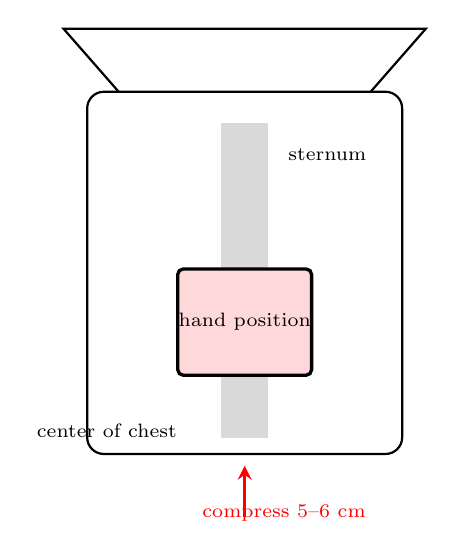
\begin{tikzpicture}[scale=1.0, >=stealth]
  \draw[thick, rounded corners=6pt] (-2.0,-2.6) rectangle (2.0,2.0);
  \draw[thick] (-1.6,2.0) -- (-2.3,2.8) -- (2.3,2.8) -- (1.6,2.0);
  \fill[gray!30] (-0.3,-2.4) rectangle (0.3,1.6);
  \node at (1.05,1.2) {\scriptsize sternum};
  \draw[very thick, fill=red!15, rounded corners=2pt] (-0.85,-1.6) rectangle (0.85,-0.25);
  \node at (0,-0.92) {\scriptsize hand position};
  \draw[->, very thick, red] (0.0,-3.4) -- (0.0,-2.75);
  \node[red] at (0.5,-3.35) {\scriptsize compress 5--6 cm};
  \node at (-1.75,-2.3) {\scriptsize center of chest};
\end{tikzpicture}
\caption{Adult CPR hand placement: heel of one hand on the center of the chest (lower half of the sternum), arms straight, pushing straight down 2--2.4 inches (5--6 cm).}
\label{fig:cpr_hands}
\end{figure}

\subsection{Rescue Breaths (If Trained and Willing)}

After 30 compressions, give 2 rescue breaths:

\begin{enumerate}[leftmargin=*]
\item Open airway using head-tilt/chin-lift maneuver: Place one hand on forehead, gently tilt head back; use second hand to lift chin point upward
\item Pinch nose shut
\item Seal your mouth over theirs and give breaths that make chest rise visibly (about 1 second each)
\item If chest does not rise, reposition head and try again
\end{enumerate}
\textbf{WARNING:} \textbf{If untrained or unwilling to give breaths, perform Hands-Only CPR}: Continuous chest compressions at 100-120 bpm without stopping for breaths. This is still effective for adults whose cardiac arrest is sudden.

\begin{center}
\begin{tabular}{@{}lll@{}}
\hline
\textbf{Group} & \textbf{Compression-Breath Ratio} & \textbf{Notes} \\
\hline
Adults (single rescuer) & 30:2 & One rescuer \\
Adults (two rescuers) & 30:2 & Standard ratio \\
Children (1 year to puberty) & 30:2 & Single rescuer \\
Children (professional/rescuer pair) & 15:2 & Two rescuers \\
Infants (<1 year) & 30:2 & Single rescuer \\
Infants (two rescuers) & 15:2 & Two rescuers \\
\hline
\end{tabular}
\end{center}

\subsection{Hands-Only CPR (Compression-Only CPR)}

If you are untrained, unsure of your skills, or unwilling to give rescue breaths, perform hands-only CPR instead of doing nothing:

\begin{enumerate}[leftmargin=*]
\item Call emergency services (or have someone else call) and place the person on their back on a firm, flat surface
\item Push hard and fast in the center of the chest: at least 2 inches (5 cm) deep, at 100--120 compressions per minute, without stopping
\item Continue until professional help arrives, an AED is ready, or the person shows signs of life
\end{enumerate}

Hands-only CPR works well for a sudden, witnessed collapse in an adult (typically a cardiac cause). Rescue breaths matter more for children, infants, and adults whose arrest follows drowning, drug overdose, or prolonged respiratory distress -- if you can give breaths, do so. If you cannot, chest compressions alone are still far better than nothing. Emergency dispatchers may also talk you through hands-only compressions.

\subsection{Two-Rescuer CPR}

If a second trained rescuer is available, coordinate to maintain high-quality compressions and effective ventilation:

\begin{itemize}[leftmargin=*]
  \item \textbf{Assign roles}: One rescuer performs chest compressions; the other gives rescue breaths (with a barrier device if available) and prepares the AED
  \item \textbf{Adult ratio}: 30 compressions to 2 breaths. For a child or infant with two rescuers, the ratio is 15:2 (see the table above)
  \item \textbf{Compression pause}: The compressor stops compressions briefly while the second rescuer gives the breaths; the second rescuer watches for visible chest rise, then signals to resume compressions immediately
  \item \textbf{Rotate every 2 minutes}: Switch roles (about every 5 cycles of 30:2) to prevent compressor fatigue and loss of compression depth. Complete the switch in less than 10 seconds -- signal on a compression count (``one, two, three...'') so the fresh rescuer takes over without a long pause
  \item \textbf{AED}: The second rescuer attaches and operates the AED, keeping everyone clear during rhythm analysis and shock delivery
  \item \textbf{Infants}: Two-rescuer infant CPR uses the two-thumb encircling technique (thumbs on the sternum, fingers encircling the chest) so one rescuer can compress while the other ventilates
\end{itemize}

\subsection{Barrier Devices (Pocket Masks and Face Shields)}

Barrier devices reduce the risk of disease transmission during rescue breathing. Use one whenever available:

\begin{itemize}[leftmargin=*]
  \item \textbf{Pocket mask}: Place the mask over the person's mouth and nose (narrow end over the bridge of the nose). Tilt the head back under the mask, seal the mask against the face with both thumbs on the sides, and breathe through the one-way valve while lifting the jaw into the mask. Watch for visible chest rise
  \item \textbf{Face shield}: Lay the shield over the face with the opening over the mouth. Seal it with your hands and breathe through the central opening while maintaining the seal
  \item With two rescuers, one rescuer can maintain the mask seal (using the head-tilt and jaw-lift) while the other compresses, allowing ventilation to be delivered in rhythm without breaking hand position
  \item If no barrier device is available, perform rescue breaths without one, or fall back to hands-only CPR -- doing something is always better than nothing
\end{itemize}

\subsection{High-Quality CPR Essentials}

The survival benefit of CPR depends on how well it is performed. Focus on these quality measures:

\begin{itemize}[leftmargin=*]
  \item \textbf{Minimize interruptions}: Keep pauses in compressions under 10 seconds. Stop only for rhythm analysis, shock delivery, or role rotation
  \item \textbf{Maximize the compression fraction}: Aim to be compressing the chest more than 80\% of the total time
  \item \textbf{Full recoil}: Allow the chest to completely expand between compressions; do not lean on the chest
  \item \textbf{Correct depth and rate}: Adults 2--2.4 inches (5--6 cm) at 100--120 per minute; allow no drift from fatigue -- this is why rescuers rotate
  \item \textbf{Avoid excessive ventilation}: Give each breath over about 1 second with just enough volume to make the chest rise visibly; too much or too fast ventilation reduces blood return to the heart
  \item \textbf{Coordinate with the AED}: When the AED is analyzing or delivering a shock, compressions pause; the moment it finishes, resume compressions immediately without delay
\end{itemize}

\section{Pediatric CPR (Infants and Children)}

\subsection{Infant CPR (Under 1 Year Old)}

\subsubsection{Technique Differences}

\begin{itemize}[leftmargin=*]
  \item Use two fingers (middle and ring) on the center of the chest just below the nipple line
  \item Or use two-thumb encircling technique (for two rescuers): thumbs side-by-side on lower third of sternum, fingers around back supporting the chest
  \item Compression depth: about 1.5 inches (4 cm) -- one-third the depth of the chest
  \item Rate: 100-120 bpm
  \item Rescue breaths: Cover both mouth AND nose when giving breaths (small mouth-to-mouth seal)
\end{itemize}

\subsection{Child CPR (1 Year to Puberty)}

\begin{itemize}[leftmargin=*]
  \item Use one or two hands depending on child size (one hand may suffice for smaller children)
  \item Compression depth: about 2 inches (5 cm)
  \item Rate: 100-120 bpm
  \item Follow adult compression technique otherwise
\end{itemize}

\textbf{WARNING:} \textbf{Important: Pediatric cardiac arrest is often respiratory in origin. Ensure proper airway positioning and adequate ventilation are emphasized in addition to compressions.}

\subsection{Moving a Child or Infant During CPR}

Begin CPR where you find the child or infant if the scene is safe. Move them ONLY if:

\begin{itemize}[leftmargin=*]
  \item The current location is unsafe (fire, electrical hazard, water, traffic, violence)
  \item The surface is too soft to allow effective compressions (e.g., a sagging mattress) and a firm surface is immediately available
  \item You are already moving to reach help or a family member
\end{itemize}

How to move: for an infant, support the head and neck with one hand and cradle the body with your forearm; for a child, carry them in your arms supporting the head. Minimize movement and avoid bending or twisting the neck. Once on a firm surface, resume CPR immediately. Do NOT delay compressions to reposition a child who is already on a firm, safe surface.

\section{Automated External Defibrillator (AED)}

An AED is a portable device that analyzes heart rhythm and delivers shocks if needed. Early defibrillation dramatically improves survival from ventricular fibrillation/pulseless ventricular tachycardia.

\subsection{AED Usage Steps}

\begin{enumerate}[leftmargin=*]
\item Turn on the AED (follow voice prompts)
\item Expose the person's bare chest and wipe dry if wet
\item Attach electrode pads as shown in diagram on package: upper right chest (below collarbone) and lower left side (below armpit)
\item Ensure nobody touches the person while the AED analyzes the rhythm
\item Follow AED prompts: If shock advised, ensure everyone is clear and press the shock button. If no shock advised, resume CPR immediately
\end{enumerate}
\begin{figure}[h]
\centering
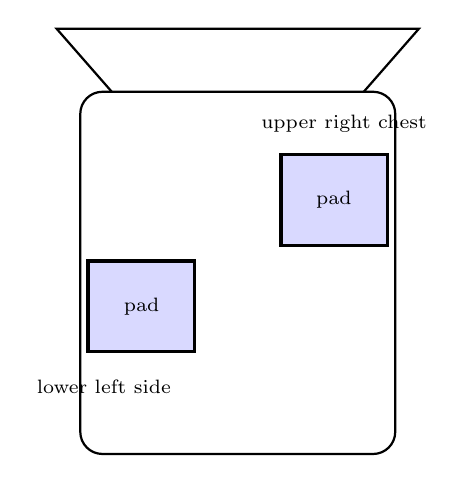
\begin{tikzpicture}[scale=1.0, >=stealth]
  \draw[thick, rounded corners=8pt] (-2.0,-2.6) rectangle (2.0,2.0);
  \draw[thick] (-1.6,2.0) -- (-2.3,2.8) -- (2.3,2.8) -- (1.6,2.0);
  \draw[very thick, fill=blue!15] (0.55,1.2) rectangle (1.9,0.05);
  \node at (1.22,0.63) {\scriptsize pad};
  \draw[very thick, fill=blue!15] (-1.9,-0.15) rectangle (-0.55,-1.3);
  \node at (-1.22,-0.73) {\scriptsize pad};
  \node at (1.35,1.6) {\scriptsize upper right chest};
  \node at (-1.7,-1.75) {\scriptsize lower left side};
\end{tikzpicture}
\caption{AED electrode pad placement: one pad on the upper right chest below the collarbone, the other on the lower left side below the armpit.}
\label{fig:aed_pads}
\end{figure}

\quicknote{\textbf{Defibrillation Priority}: For a witnessed collapse where someone can grab an AED immediately, use the AED as soon as possible, even before beginning extensive CPR. Unwitnessed collapse starts with CPR first.}

\textbf{WARNING:} \textbf{Pacemakers}: If you see a hard lump under the skin on the chest (pacemaker or ICD), avoid placing the electrode pad directly over it. Place the pad at least 1 inch away.

\quicknote{\textbf{Children}: For children under 8 years or under 25 kg (55 lbs), use pediatric pads or a dose-attenuating device if available. If only adult pads are available, use them -- delivering a shock is preferable to no shock. For children under 1 year, an AED may be used with pediatric pads or a dose-attenuator if available.}

\subsubsection{AED Use in Infants}
For infants under 1 year old:
\begin{itemize}
  \item Preferred: Use a pediatric AED with child-sized pads or a dose-attenuator that reduces the shock energy
  \item If pediatric AED is not available: Use a standard AED with adult pads -- do not withhold defibrillation
  \item Pad placement: anterior--posterior (one pad on center of chest, one on center of back) is preferred for infants if using adult pads, to prevent pads from touching
  \item If pads would touch on the front and back, use the anterior--posterior placement rather than risking contact
\end{itemize}
\textbf{WARNING}: Never use a pediatric dose-attenuator with an AED designed only for adult use, and never use adult pads on an infant if pediatric pads are available -- the shock energy may be excessive.

\subsection{Special Situations and Pad Placement}

\begin{itemize}[leftmargin=*]
  \item \textbf{Medication patches}: If a patch (e.g., nitroglycerin, nicotine, pain reliever) is on the chest where a pad will go, remove it with a gloved hand and wipe the skin dry before attaching the pad -- patches can conduct electricity and cause burns during shock delivery
  \item \textbf{Wet chest}: Dry the chest thoroughly before attaching pads; pads will not stick to wet or sweaty skin
  \item \textbf{Dense chest hair}: If the pads do not stick well, shave the area quickly with the razor included in the AED kit, or press the pads firmly through the hair. Do not delay shocks for extensive shaving
  \item \textbf{Jewelry and piercings}: Leave jewelry and piercings in place unless they sit directly under a pad; move the pad slightly. Do not waste time removing jewelry
  \item \textbf{Pacemaker or ICD}: If you see or feel a hard lump under the skin on the chest, place the pad at least 1 inch away from it (see the warning above)
  \item \textbf{Water}: Do not use an AED on a person lying in water or a puddle -- move them to a dry surface before attaching pads (and before CPR)
  \item \textbf{Alternate pad positions}: If standard pad placement is not possible (e.g., an implanted device or injury in the way), use the anterior--posterior position: one pad on the front of the chest and the other on the back between the shoulder blades
\end{itemize}

\section{Airway Management in First Aid}

Maintaining a patent airway is essential in any unconscious patient.

\subsection{Head-Tilt/Chin-Lift Maneuver}

Used to open the airway in an unresponsive person without suspected spinal injury.

\begin{enumerate}[leftmargin=*]
\item Place hand on forehead and apply firm, backward pressure
\item Use fingertips under bony part of lower jaw and lift forward
\item This tilts the head back and lifts tongue away from posterior pharyngeal wall
\end{enumerate}
\textbf{WARNING:} \textbf{Suspected Spinal Injury}: Use the Jaw-Thrust Maneuver instead: place hands on either side of head, grasp angles of mandible, and lift forward WITHOUT tilting the head. Maintain manual in-line stabilization of the neck throughout.

\subsection{Recovery Position}

See Section~\ref{sec:recovery_position} in Chapter~\ref{ch:basic_principles} for detailed instructions. Essential for maintaining airway patency in breathing but unconscious persons.

\section{Choking Management}

Conscious choking requires immediate intervention to relieve airway obstruction.

\subsection{Conscious Adult or Child Over 1 Year}

\begin{enumerate}[leftmargin=*]
  \item Ask ``Are you choking?'' If yes, encourage coughing if they can still cough, speak, or breathe (this indicates partial obstruction)
  \item If they cannot cough, speak, or breathe (severe obstruction), begin Heimlich maneuver (abdominal thrusts)
  \item Stand behind the person, wrap arms around their waist, make fist with one hand, grasp it with other, place thumb side just above navel
  \item Give quick, upward and inward thrusts until object is expelled or person becomes unconscious
\end{enumerate}
\textbf{WARNING:} \textbf{Do not perform abdominal thrusts on pregnant women or obese persons. Use chest thrusts instead: Place heel of hand on center of breastbone, give quick inward and upward thrusts.}

\subsection{Conscious Infant (Under 1 Year)}

Abdominal thrusts are dangerous for infants. Use back blows combined with chest thrusts:

\begin{enumerate}[leftmargin=*]
\item Support infant face-down along forearm, head lower than chest, support head with hand
\end{enumerate}
\begin{figure}[h]
\centering
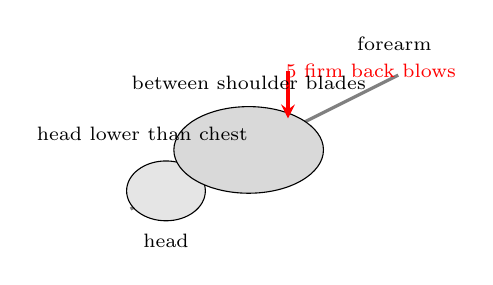
\begin{tikzpicture}[scale=1.0, >=stealth]
  \draw[very thick, gray] (0,0) -- (3.4,1.7);
  \node at (3.35,2.1) {\scriptsize forearm};
  \draw[fill=black!10] (0.45,0.23) ellipse (0.5 and 0.38);
  \draw[fill=black!15] (1.5,0.75) ellipse (0.95 and 0.55);
  \node at (0.45,-0.4) {\scriptsize head};
  \node at (0.15,0.95) {\scriptsize head lower than chest};
  \draw[->, very thick, red] (2.0,1.75) -- (2.0,1.15);
  \node[red] at (3.05,1.75) {\scriptsize 5 firm back blows};
  \node at (1.5,1.6) {\scriptsize between shoulder blades};
\end{tikzpicture}
\caption{Infant choking: hold the infant face-down along your forearm with the head supported and lower than the chest, then give 5 firm back blows between the shoulder blades.}
\label{fig:infant_backblows}
\end{figure}

\begin{enumerate}[leftmargin=*]
\item Give up to 5 firm back blows between shoulder blades with heel of hand
\item If object not expelled, turn infant face-up along forearm, support head, keep head lower than chest
\item Give up to 5 chest thrusts using two fingers on lower third of sternum (same position as compressions), pressing down about 1.5 inches
\item Alternate 5 back blows and 5 chest thrusts until object expelled or infant becomes unconscious
\end{enumerate}
\subsection{Unconscious Person (Adult, Child, or Infant)}

Lower the person carefully to the ground and begin CPR starting with chest compressions. Before rescue breaths, check the mouth for visible object; if seen, remove with finger sweep. Attempt breath; if unsuccessful, reposition head and try again. Continue CPR cycle until help arrives or object dislodges.

\medskip\noindent\textbf{CPR Quick Reference Summary.}
\begin{center}
\begin{tabularx}{\textwidth}{@{}>{\raggedright\arraybackslash}l>{\raggedright\arraybackslash}X>{\raggedright\arraybackslash}X@{}}
\hline
\textbf{Parameter} & \textbf{Adult} & \textbf{Infant/Child} \\
\hline
Compression Depth & 2-2.4 inches (5-6 cm) & 1.5-2 inches (4-5 cm) \\
Compression Rate & 100-120 bpm & 100-120 bpm \\
Compression Technique & Both hands stacked (heel on heel) & Two fingers (infant) / One or two hands (child) \\
Ratio (Single Rescuer) & 30:2 & 30:2 \\
Ratio (Two Rescuers Children) & 30:2 & 15:2 \\
\hline
\end{tabularx}
\end{center}

\section{Special Considerations}

\subsection{Dental Work and Dentures}

If dentures are loose during rescue breaths, remove them to get a better seal. If tightly fitted, leave in place as they may help form the seal.

\subsection{Person in Water (Water Rescue CPR)}

For drowning victims, provide rescue breathing promptly after removing from water. Perform 5 initial cycles of CPR (about 2 minutes) before calling for help if alone and witnessed. Prioritize rapid extrication and ventilation.

\subsection{Suspected Stroke}

Recognize FAST: Face drooping, Arm weakness, Speech difficulty, Time to call emergency services. While waiting, keep person comfortable, do not give food or drink, monitor breathing, and be prepared to initiate CPR if they become unresponsive.

\section{When Professional Help Arrives}

\begin{itemize}[leftmargin=*]
  \item Report what you observed (collapse time, CPR started/stopped times, AED usage/shocks delivered)
  \item Describe any interventions you performed
  \item Inform about medication known history if available
  \item Do not stop CPR unless directed by medical personnel or the person shows signs of life (movement, normal breathing, responsiveness)
\end{itemize}

\section{Review Questions}

\begin{enumerate}[leftmargin=*]
\item How do you locate the correct hand position for adult chest compressions, and what is the recommended depth and rate?
\item What is the correct compression-to-ventilation ratio for a single rescuer performing CPR on an adult? On an infant?
\item Why is the head-tilt/chin-lift not used when a spinal injury is suspected, and what replaces it?
\item When should a child or infant be moved (not left where they are) during CPR, and how?
\item What does a shockable rhythm mean for AED use, and what should you do if the AED does not advise a shock?
\item How does choking relief differ between an infant and an adult?
\end{enumerate}
\section{Skill Practice: CPR and Airway}

\begin{enumerate}[leftmargin=*]
\item Check scene safety and demonstrate the responsive and unresponsive checks
\item Call for help and ask for an AED (simulate)
\item Demonstrate head-tilt/chin-lift and open the airway
\item Practice 5 cycles of 30:2 chest compressions and rescue breaths on a manikin or model (check depth and rate with a partner or timer)
\item Demonstrate the jaw-thrust technique for a suspected spinal injury
\item Show AED pad placement from memory on a volunteer or diagram
\item Practice the Heimlich maneuver on a partner using appropriate force
\item Practice infant back blows and chest thrusts on a doll or rolled towel
\end{enumerate}
\index{cardiopulmonary resuscitation (CPR)}
\index{chest compressions}
\index{rescue breaths}
\index{automated external defibrillator (AED)}
\index{adult CPR}
\index{pediatric CPR}
\index{infant CPR}
\index{Heimlich maneuver}
\index{choking relief}
\index{airway management}
\index{jaw-thrust maneuver}
\index{head-tilt/chin-lift}
\index{stroke recognition}
\index{drowning response}
\index{defibrillation}
\index{hands-only CPR}
\index{compression-only CPR}
\index{two-rescuer CPR}
\index{pocket mask}
\index{face shield}
\index{barrier devices}
\index{high-quality CPR}